\section{Query Recommendation}


\begin{frame}{Query Recommendation}

Suitable refinements to an initial query

\end{frame}


\begin{frame}{Query Recommendation on Intranets}

Document collection on Intranet:
\begin{itemize}
	\item relatively small
	\item changes less frequently (than Internet)
	\item more limited context of search (than Internet) \newline
\end{itemize}

Methods for Query Recommendation on Intranets:
\begin{itemize}
	\item concept hierarchy
	\item search logs
\end{itemize} 

\end{frame}


\begin{frame}{The Concept Hierarchy Model (CHM)}

What is a concept?
\begin{itemize}
	\item keyword
	\item phrase
	\item n-grams \newline
\end{itemize}

Concept Hierarchy:
\begin{itemize}
	\item created from a document collection
	\item used for ranking terms according to the strength of their links to the query within the hierarchy
\end{itemize}

\end{frame}


\begin{frame}{Subsumption Hierarchy for REsult Clustering (SHReC)}

Use term co-occurence to build a subsumption hierarchy tree \newline

x subsume y when:
\[
	df(x) > df(y) \land d(x \land y) / df(y) \geq \alpha
\]
where:
\begin{itemize}
	\item \emph{df} is the document frequency function
	\item \emph{$ \alpha $} is the strength of subsumption \newline
\end{itemize}

$ G_{SHReC} = (V, E, w) $:
\begin{itemize}
	\item \emph{V}, set of nodes containing all unique concepts + a special node 'SHReC root'
	\item $ E \subseteq V \times V $, set of directed edges
	\item $ w : E \rightarrow (0..1] $, weighting function 
\end{itemize}

\end{frame}


\begin{frame}{SHReC - example}

Terms ranked by:
\[
	w(x, y) = d(x \land y) / df(x)
\]

\begin{figure}
	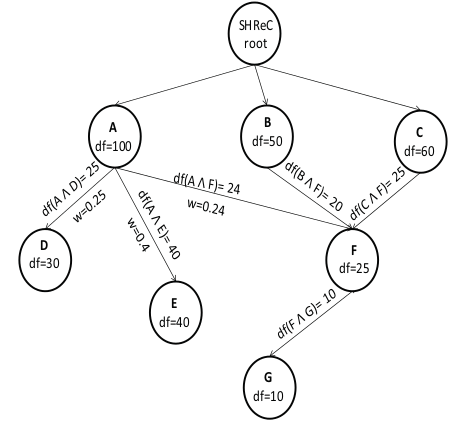
\includegraphics[scale=0.4]{img/SHReC-Example.png}
\end{figure}

\end{frame}


\begin{frame}{Query Recommendation using Search Logs}

Types:
\begin{itemize}
	\item local (based only on each user's previous searches)
	\item global (based on all previous searches) \newline
\end{itemize}

Query Flow Graph
\begin{itemize}
	\item state-of-the-art log-based query recommender
	\item directed graph:
		\begin{itemize}
			\item nodes contain queries
			\item edges represent query refinements 
		\end{itemize}
\end{itemize}

\end{frame}


\begin{frame}{Adaptation of CHM with Search Logs}

Concept Hierarchy discovers relationships between terms based on statistical analysis, giving a conceptual view \newline

Search Logs provide a conceptual view based on collective user intelligence \newline

Two complementary conceptual views on the same search domain
$ \Rightarrow $
Adapt the CHM with user interactions derived from Search Logs

\end{frame}


\begin{frame}{Adapting SHReC with Search Logs - algorithm}

\begin{scriptsize}
	\begin{columns}
		\begin{column}[l]{0.5\textwidth}
			$ G_{SHReC} = (V, E, w) $ \\
			$ G_{normSHReC} $, normalised SHReC \\
			$ R = \{r_{1}, ..., r_{n}\} $, reformulations \\
			$ r_{i} = x \rightarrow y $, query 'x' reformulated as query 'y' \\
			$ lw(r_{i}) = logWeight(x, y) = \frac{totalFreq(x \rightarrow y)}{totalFreq(x \rightarrow *)} $ \\
		\end{column}

		\begin{column}[l]{0.5\textwidth}
			\begin{tabbing}
				$ G_{normSHReC} = norm(G_{SHReC}) = (V, E, w_{adapted}, w') $ \\
				for \= each $ r_{i} \in R $ do \\
				\>	if \ \= $ x \in V $ and $ y \in V $ then \\
				\>	\>	$ G_{normSHReC}.updateweights(x, y, lw(r_{i})) $ \\
				\>	\>	$ w_{adapted}(x, y) = w'(r_{i}) + lw(r_{i}) $ \\
				\>	else if $ x \in V $ and $ y \notin V $ then \\
				\>	\>	$ G_{normSHReC}.addDescendant(x, y, lw(r_{i})) $ \\
				\>	\>	$ w_{adapted}(x, y) = lw(r_{i}) $ \\
				\>	else if $ x \notin V $ and $ y \in V $ then \\
				\>	\>	$ G_{normSHReC}.addAscendant(y, x, lw(r_{i})) $ \\
				\>	\>	$ w_{adapted}(x, y) = lw(r_{i}) $ \\
				\>	else \\
				\>	\>	$ G_{normSHReC}.add(y, x, lw(r_{i})) $ \\
				\>	\>	$ w_{adapted}(x, y) = lw(r_{i}) $ \\
				\>	end if \\
				end for \\
			\end{tabbing}
		\end{column}
	\end{columns}
\end{scriptsize}

\end{frame}


\begin{frame}{Adapting SHReC with Search Logs - example}

\begin{figure}
	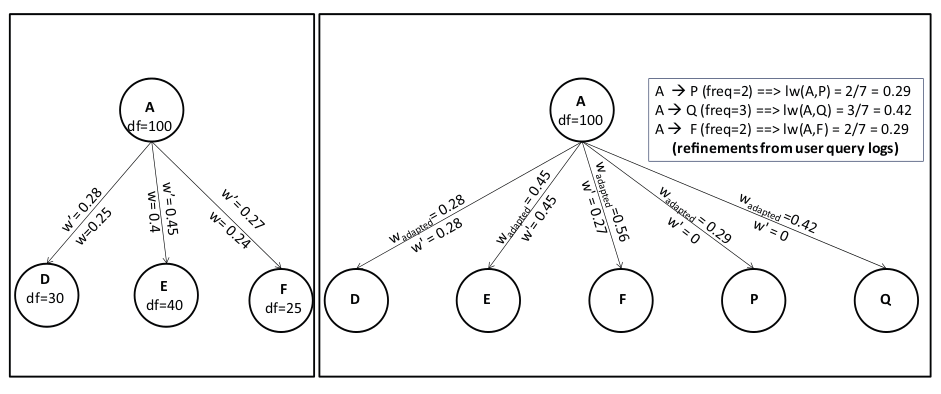
\includegraphics[scale=0.3]{img/A-SHReC-Example.png}
\end{figure}

\end{frame}


\begin{frame}{SHReC Results}

Adaptive SHReC is more efficient than QFG, which is more efficient that static SHReC \newline

Users will benefit more from the models when all log refinements are used for adaptation rather than only those with clicks

\end{frame}

